\chapter{Cablaggio, Switching e Fabric di Rete}

\section{Il Mezzo Fisico: Rame e Fibra Ottica}
La rete è il sistema vascolare del datacenter. L'evoluzione della densità di traffico ha segnato il progressivo abbandono del rame a favore della fibra ottica.

\subsection{Cavi in Rame ed Ethernet}
Storicamente, i data center si basavano pesantemente sul rame (es. i vecchi cavi \textbf{Cat 5} o Cat 5e che limitavano le velocità a 100 Mbps o 1 Gbps). I limiti fisici del rame (diafonia e attenuazione del segnale) e la necessità di gestire un preciso \textit{pin-out} per l'allineamento dei contatti hanno reso sempre più complessa l'evoluzione. 
Oggi, il tradizionale cavo in rame (standard Ethernet con connettore RJ45) è confinato al limite pratico dei \textbf{10 Gbps (Cat 6A)}. Andare oltre con standard come Cat 7 o Cat 8 risulta impraticabile: i cavi diventano spessi, rigidi e difficili da gestire (il cosiddetto \textit{cable management} è vitale, poiché un cablaggio disordinato blocca il flusso d'aria e distrugge l'efficienza termica del rack).

\subsection{Fibra Ottica e Transceiver}
\begin{figure}[H]
    \centering
    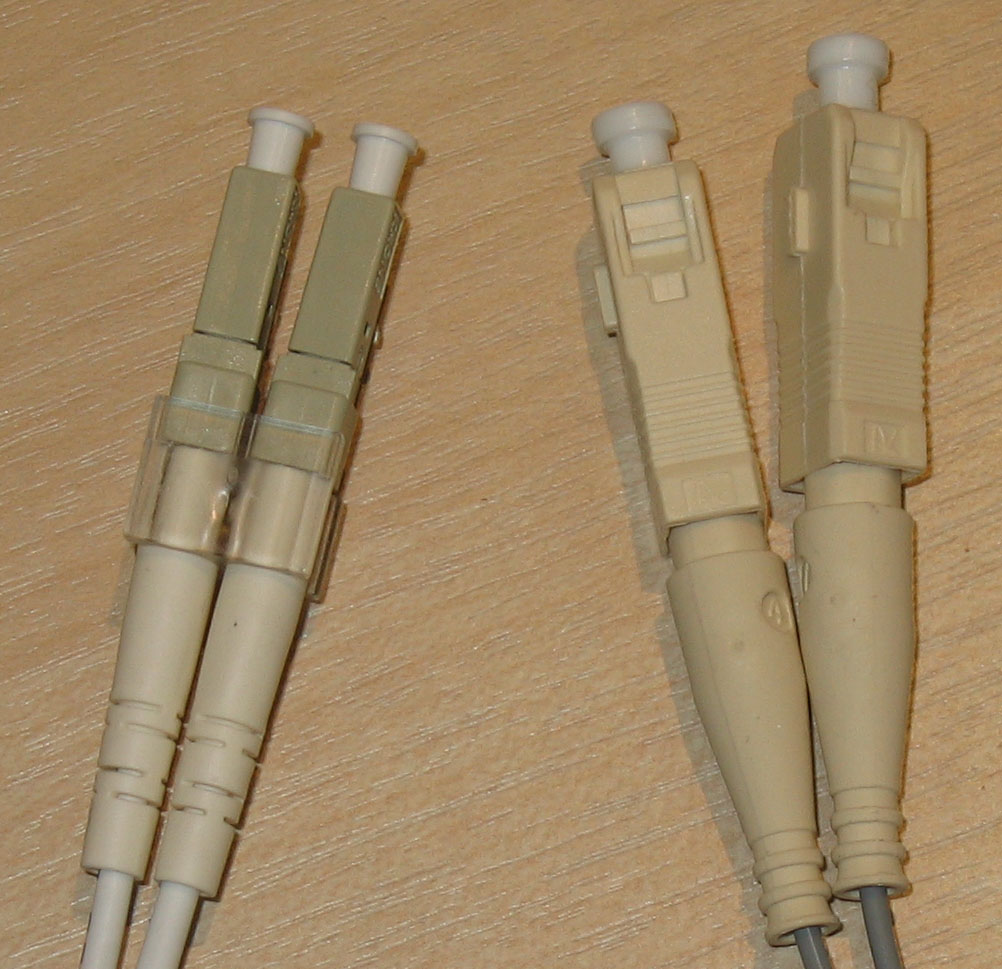
\includegraphics[width=0.6\textwidth]{images/fiber_connectors.jpg}
    \caption{Connettori ottici in fibra (LC e SC a confronto).}
\end{figure}
La trasmissione ottica azzera la dissipazione termica e aumenta vertiginosamente la banda, ma richiede l'uso di \textbf{transceiver} (moduli hot-swappable) per convertire il segnale elettrico in ottico. L'evoluzione di questi moduli ha definito le velocità del datacenter:
\begin{itemize}
    \item \textbf{SFP28:} Standard per porte server a 25 Gbps (singola lane).
    \item \textbf{Famiglia QSFP (Quad SFP):} Usa 4 lane interne. Include QSFP+ (40G), \textbf{QSFP28} (100G, standard per uplink), fino ai moderni \textbf{QSFP56} (200G) e \textbf{QSFP-DD} (fino a 800G).
\end{itemize}
Il salto prestazionale oltre i 100G non è avvenuto aggiungendo cavi, ma cambiando modulazione del segnale da \textbf{NRZ} (1 bit per simbolo) a \textbf{PAM4} (2 bit per simbolo, raddoppiando la banda alla stessa frequenza). I moduli utilizzano codici colore standardizzati incisi sul corpo (es. blu per monomodale, nero/grigio per multimodale).

Le fibre si dividono in due grandi famiglie:
\begin{itemize}
    \item \textbf{Multimodale (OM):} core più largo (50 $\mu$m), permette più rimbalzi dei fotoni. Ha distanze operative brevi (fino a $\sim$100-300 m) ma costi inferiori. È lo standard dominante \textit{all'interno} del datacenter.
    \item \textbf{Monomodale (OS):} core sottilissimo (9 $\mu$m), permette un unico percorso rettilineo. Ideale per collegamenti metropolitani a lungo raggio (fino a 40 km).
\end{itemize}

\section{Architettura interna degli Switch}
\begin{figure}[H]
    \centering
    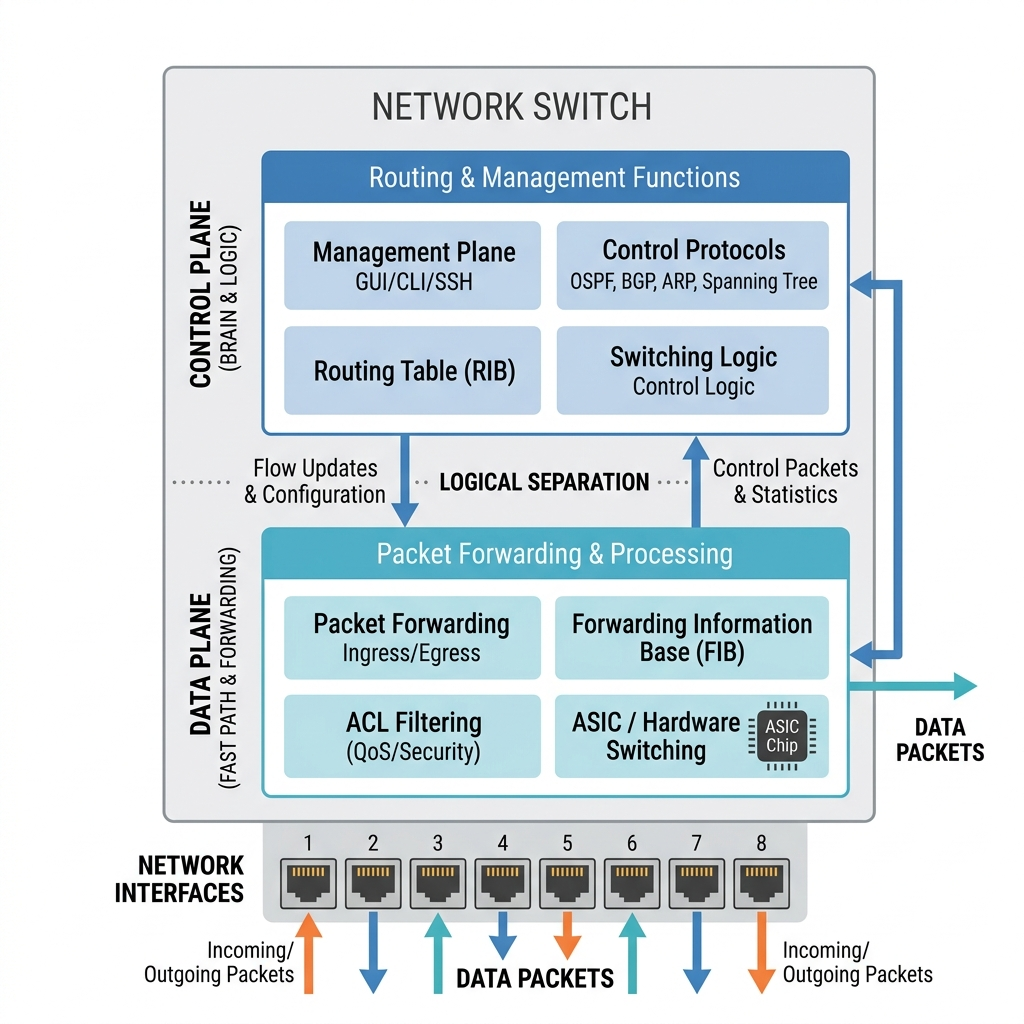
\includegraphics[width=0.7\textwidth]{images/network_planes.png}
    \caption{Architettura logica: separazione tra Control Plane e Data Plane in un dispositivo di rete.}
\end{figure}
In passato, l'architettura di rete dominante si basava su enormi \textit{chassis modulari} proprietari (es. i grandi switch core di Cisco), costosi e difficili da scalare gradualmente. Lo switch moderno, spinto dalle esigenze iperscalabili del cloud, ha abbandonato gli chassis a favore del \textbf{Fixed Form Factor} (1U o 2U), spesso definito \textit{White-box switch}.

\subsection{Software-Defined Networking (SDN) e SONiC}
\begin{figure}[H]
    \centering
    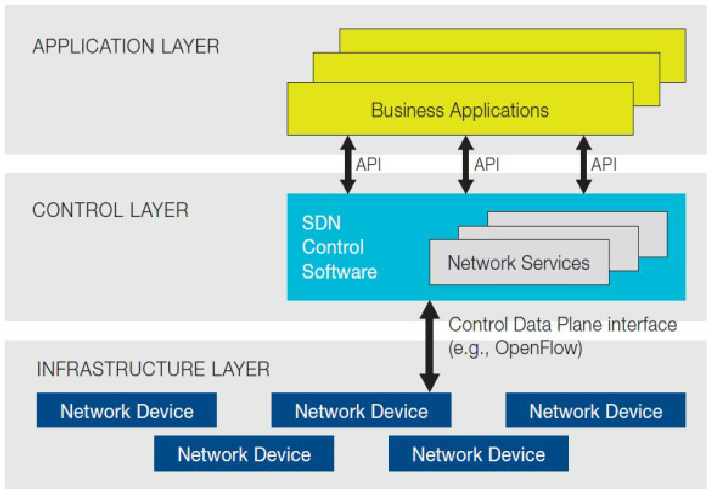
\includegraphics[width=0.7\textwidth]{images/sdn.png}
    \caption{Modello SDN: l'intelligenza di rete viene astratta dall'infrastruttura fisica sottostante.}
\end{figure}
La grande rivoluzione è stata la separazione concettuale in due piani:
\begin{enumerate}
    \item \textbf{Data Plane (Piano Dati):} hardware dedicato (spesso ASIC commodity, es. chip Broadcom) che si occupa di inoltrare pacchetti (\textit{forwarding}) a velocità \textit{line-rate}. Gli switch moderni sono \textit{non-blocking}, ovvero capaci di inoltrare traffico su tutte le porte simultaneamente senza colli di bottiglia.
    \item \textbf{Control Plane (Piano di Controllo):} un vero e proprio computer (spesso con CPU x86 e sistema operativo Linux) che gestisce la logica di rete (routing come BGP, policy, ecc.).
\end{enumerate}
\begin{figure}[H]
    \centering
    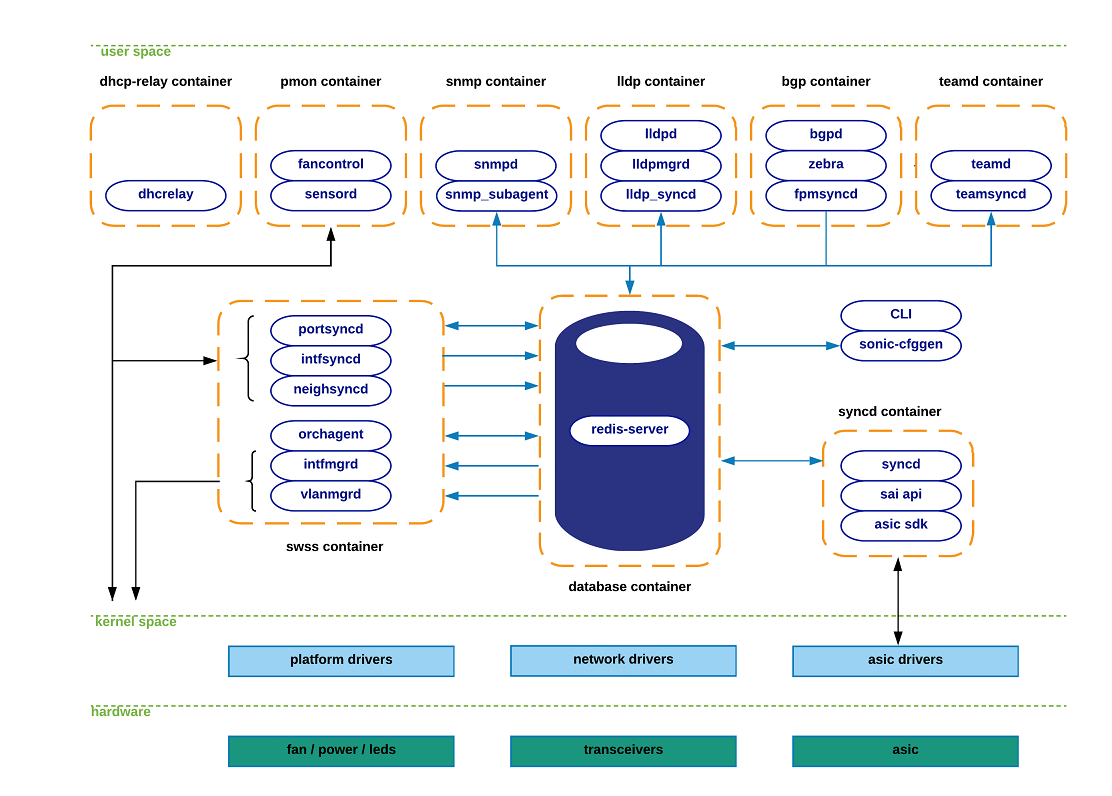
\includegraphics[width=0.7\textwidth]{images/sonic.png}
    \caption{Architettura SONiC: ogni funzione di rete gira nel proprio container Docker comunicando tramite Redis.}
\end{figure}
La disaggregazione hardware-software ha portato alla nascita di Sistemi Operativi di Rete (NOS) open source come \textbf{SONiC} (Software for Open Networking in the Cloud, creato da Microsoft). Avviato tramite il bootloader ONIE, SONiC tratta lo switch come un server standard, eseguendo ogni demone di routing all'interno di \textit{container Docker} isolati.

\section{Topologie di Rete: Dal 3-Tier allo Spine-and-Leaf}
Storicamente, i datacenter adottavano una topologia \textbf{3-tier} (Access, Distribution, Core), ottimizzata per il traffico \textbf{Nord-Sud} (client-server). 
I collegamenti ridondanti creavano inevitabilmente loop fisici. Se un pacchetto broadcast iniziava a ciclare, innescava un catastrofico \textbf{Broadcast Storm} in grado di paralizzare l'intero datacenter in pochi secondi. Per evitarlo si utilizzava il protocollo \textbf{STP (Spanning Tree Protocol)}, che disabilitava preventivamente i link fisici ridondanti. I difetti dell'STP erano molteplici: enormi sprechi di banda (fino al 50\% dei cavi posati rimaneva dormiente) e lenti tempi di convergenza in caso di guasto (i ricalcoli della topologia bloccavano momentaneamente il traffico).

Oggi, l'esplosione dei microservizi, del cloud e dell'IA ha reso assolutamente dominante il traffico \textbf{Est-Ovest} (server-to-server). La topologia standard dei moderni data center è diventata la \textbf{Spine-and-Leaf} (derivata dalle reti di \textit{Clos}):

\begin{figure}[H]
    \centering
    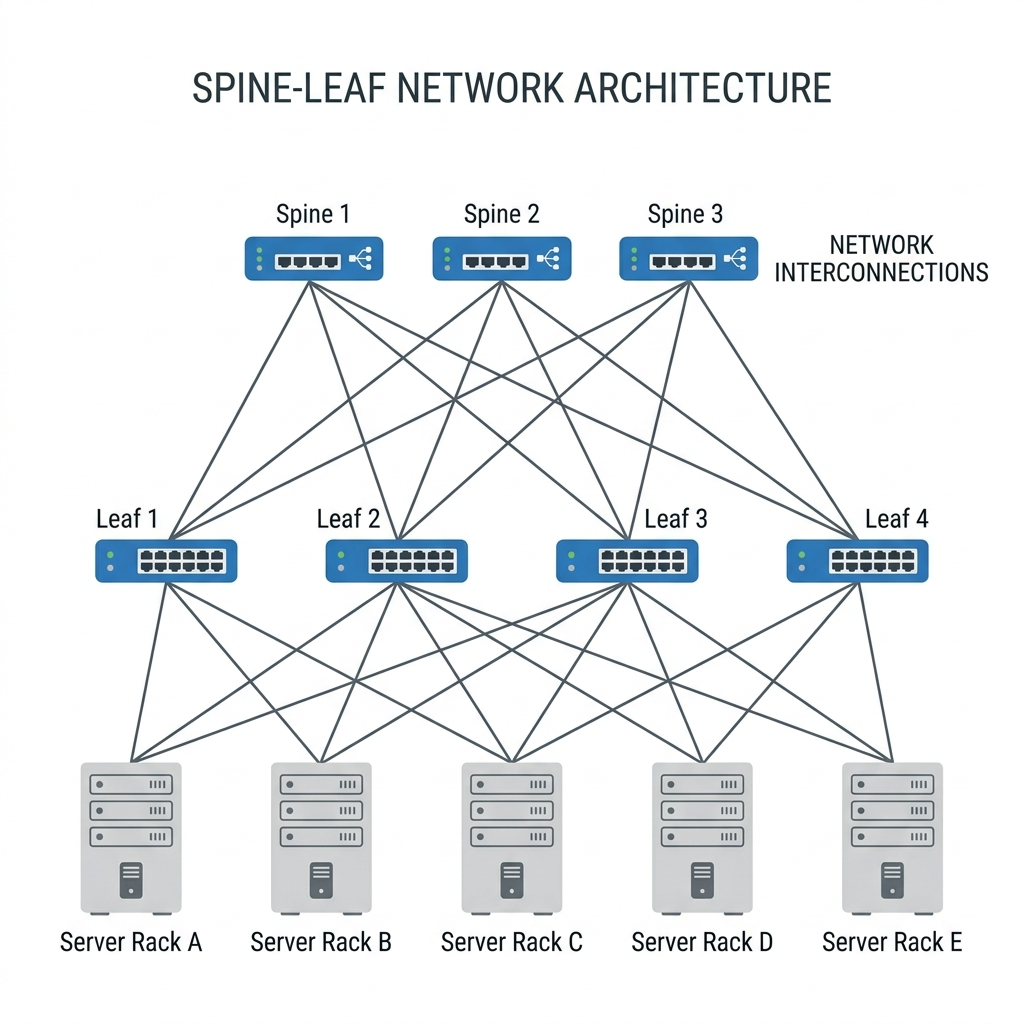
\includegraphics[width=0.8\textwidth]{images/spine_leaf_arch.png}
    \caption{Architettura Spine-Leaf: connessione Full-Mesh tra livello Leaf e livello Spine.}
\end{figure}

L'architettura si sviluppa su due livelli fisici rigorosi:
\begin{itemize}
    \item \textbf{Leaf Layer (Accesso):} Costituito dagli switch ToR (Top-of-Rack). I server fisici si collegano \textit{solo} a questi switch. A loro volta, gli switch Leaf \textbf{non sono mai collegati tra loro}.
    \item \textbf{Spine Layer (Backbone):} Il livello centrale di aggregazione. Ogni singolo switch Leaf possiede almeno un collegamento uplink in fibra verso \textbf{ogni} singolo switch Spine (creando una configurazione \textit{Full-Mesh} tra i due livelli). Anche gli switch Spine \textbf{non si parlano mai direttamente tra di loro}.
\end{itemize}

\begin{tipbox}[Vantaggi e Oversubscription]
\begin{itemize}
    \item \textbf{Latenza Deterministica:} Ogni server comunica con un qualsiasi altro server impiegando esattamente lo stesso numero di salti (1 hop logico: \textit{leaf $\rightarrow$ spine $\rightarrow$ leaf}).
    \item \textbf{ECMP (Equal-Cost Multi-Path):} Senza i tradizionali loop fisici, l'STP viene sostituito dal routing L3. Il traffico viene bilanciato uniformemente (load balancing) su \textit{tutti} gli uplink disponibili. Se uno switch Spine fallisce, la rete si degrada solo frazionalmente in banda, ma non si interrompe.
    \item \textbf{Oversubscription Ratio:} Il rapporto tra banda totale di downlink (verso i server) e uplink (verso gli Spine). Un tipico cloud usa rapporti 3:1. Gli ambienti HPC o AI esigono un rapporto \textbf{1:1} (detto \textit{Non-blocking}), garantendo che tutti i server possano trasmettere al massimo contemporaneamente senza colli di bottiglia.
\end{itemize}
\end{tipbox}

\section{Segmentazione e Virtualizzazione della Rete}
\subsection{VLAN (Virtual LAN)}
L'header Ethernet classico contiene un indirizzo MAC di destinazione (6 byte), un MAC sorgente (6 byte) e un campo EtherType (2 byte). Le VLAN (standard IEEE 802.1Q) permettono di suddividere una rete fisica in più domini di broadcast logici, inserendo un tag di 4 byte subito dopo il MAC sorgente. 
Questo tag 802.1Q include un campo TPID (che indica la presenza della VLAN) e un TCI, il quale a sua volta contiene 3 bit per la priorità (QoS) e \textbf{12 bit per l'identificativo VLAN (VID)}. Essendo l'ID VLAN lungo esattamente 12 bit, il limite teorico invalicabile è di \textbf{4094 reti} utilizzabili ($2^{12}-2$), un numero assolutamente insufficiente per i moderni cloud provider multi-tenant che devono ospitare centinaia di migliaia di reti isolate.

\subsection{VXLAN e Overlay}
Per superare la rigidità architetturale e il limite di 4096 reti delle VLAN tradizionali, il datacenter cloud moderno usa \textbf{VXLAN (Virtual eXtensible LAN)}. È un protocollo di \textit{overlay} (Mac-in-UDP) che incapsula interi pacchetti Layer 2 (Ethernet) all'interno di pacchetti di trasporto Layer 3 (UDP/IP). 
Questo innalza il limite a \textbf{16 milioni di reti virtuali isolate} (grazie a un identificativo VNI a 24 bit) e permette di creare domini di broadcast Layer 2 arbitrari su un'infrastruttura fisica di routing Layer 3. Ciò significa che due macchine virtuali possono credere di essere collegate allo stesso switch fisico (stessa subnet L2), anche se si trovano in due rack fisicamente distanti instradati in L3.

\section{Fabric ad Alte Prestazioni (HPC e AI)}
In contesti HPC e di addestramento AI, dove la computazione è pesantemente distribuita e sincronizzata, la latenza introdotta dallo stack TCP/IP Ethernet (tipicamente $\sim$70 $\mu$s) è inaccettabile.

In questi scenari domina \textbf{InfiniBand}, una rete che offre latenze di 1-3 $\mu$s. Il segreto è l'implementazione del protocollo \textbf{RDMA (Remote Direct Memory Access)}, che permette a un server di scrivere direttamente nella memoria RAM di un altro server scavalcando completamente l'intervento della CPU e del sistema operativo ricevente.
Oggi, RDMA è disponibile anche su reti Ethernet avanzate tramite il protocollo \textbf{RoCE} (RDMA over Converged Ethernet).

\begin{definitionbox}[Full Fat Tree]
Per evitare l'\textit{overbooking} (sovraccarico degli uplink) critico per l'HPC, si usa la topologia \textbf{Full Fat Tree}: una struttura non-bloccante in cui la larghezza di banda verso i livelli superiori è esattamente pari a quella dei livelli inferiori, garantendo comunicazioni senza strozzature.
\end{definitionbox}
